\chapter{User Workflow}
\label{chapter:ch5_user_workflow}

This chapter documents the operator workflow of the prototype via the web frontend: how to start the system, instantiate and wire the module graph, activate modules, calibrate the robot-mounted stereo camera, and author and execute commands for the two evaluated use cases (welding and pick-and-place).
The frontend actions correspond to the orchestration behavior described in \autoref{sec:ch3_ui_orchestration}, and the instantiated module configuration follows \autoref{fig:runtime_full}.

Build and installation steps for the submitted code snapshot are described in \autoref{appendix:source_code}.
The delivered artifact files (Charuco PDF, camera mount CAD, pen CAD/firmware, scene CAD/registry, and CBun sources) are summarized in \autoref{appendix:artifacts};
the prototype hardware setup (including the stereo camera) is described in \autoref{sec:ch4_physical_setup}.

% ----------------------------------------------------------
\section{Preconditions and environment}
\label{sec:ch5_preconditions}

\minihead{Physical setup.}
The workflow assumes:
\begin{itemize}
  \item Kassow robot with a stereo camera rigidly mounted to the tool flange (mount CAD in \autoref{appendix:camera_mount_cad}; camera hardware in \autoref{subsec:ch4_hw_camera}).
        The cable from the camera is routed along the robot arm so that it does not occlude the camera, interfere with motion, or get pinched.
  \item A computer connected to the camera (USB) and to the robot controller (Ethernet). A direct wired connection and static IP addressing in a common subnet are recommended (avoid wireless connection).
  \item The tracked pen assembled, flashed, charged, and available over BLE as ``\type{3D Pen}'' (\autoref{appendix:pen_artifacts}).
  \item For calibration: a Charuco board printed at 100\,\% scale and mounted flat on a rigid backing (\autoref{appendix:charuco}).
  \item For the use cases: fiducial-tagged box objects visible to the camera (CAD \autoref{appendix:scene_cad}, registry \autoref{appendix:scene_registry}).
\end{itemize}

\minihead{Software setup.}
This chapter assumes the installed runtime layout under \path{binaries/} as described in \autoref{appendix:source_code}.

\minihead{Robot-side boundary.}
The Aergo CBun is assumed installed and enabled on the robot controller (sources/build notes in \autoref{appendix:cbun}).
Configuring the robot controller (network settings, CBun installation) is outside the scope of this chapter.

% ----------------------------------------------------------
\section{System startup}
\label{sec:ch5_startup}

\minihead{Start the runtime.}
From the installed layout (\autoref{appendix:source_code}), start the runtime by running the core executable with the \type{modules} and \type{data} directories as arguments:
\begin{verbatim}
cd binaries
.\core.exe modules data
\end{verbatim}
Then open \url{http://localhost:8080} in a browser.

% ----------------------------------------------------------
\section{Instantiate the module graph}
\label{sec:ch5_graph_setup}

\begin{figure}[H]
  \centering
  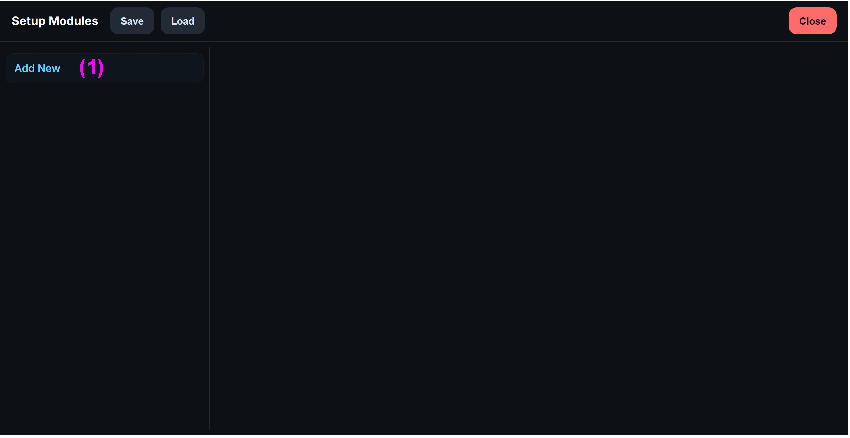
\includegraphics{img/ch5_user_workflow/01_initial_screen.pdf}
  \caption[Setup Modules view]{\emph{Setup Modules} view: the initial screen after starting the runtime.}
  \label{fig:ch5_initial_screen}
\end{figure}

\minihead{Goal.}
Create the module instances corresponding to \autoref{fig:runtime_full}.

\minihead{Add modules.}
After launching the core and opening the frontend, the initial view is \emph{Setup Modules} (\autoref{fig:ch5_initial_screen}), which shows the current instantiated module list (empty at launch). 
From the \emph{Setup Modules} view, press \emph{Add New} \uicall[fig:ch5_initial_screen]{1} to open the \emph{Add Module} view.

\begin{figure}[H]
  \centering
  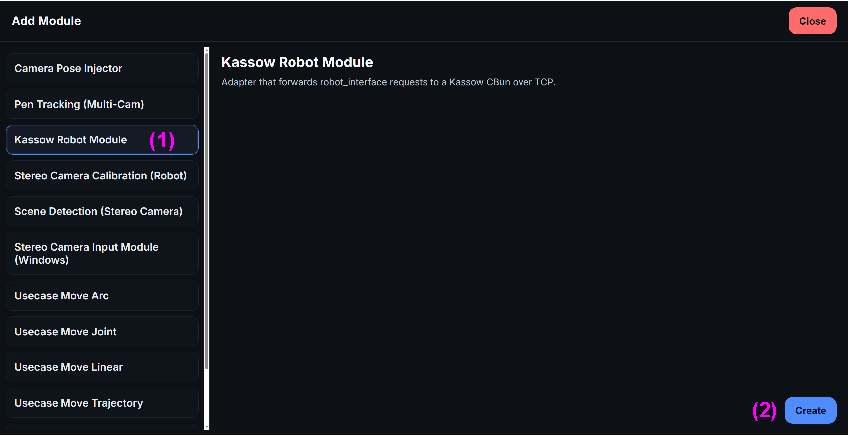
\includegraphics{img/ch5_user_workflow/02_add_robot.pdf}
  \caption[Add Module view]{\emph{Add Module} view: adding the robot module.}
  \label{fig:ch5_add_module}
\end{figure}

In the \emph{Add Module} view (\autoref{fig:ch5_add_module}), the left list shows available module types, and the right panel shows input mapping options for the selected module type. In the left list, select \emph{Kassow Robot Module} \uicall[fig:ch5_add_module]{1} and press \emph{Create} \uicall[fig:ch5_add_module]{2} to add the robot module instance.

Repeat the same steps for the following module types in the order shown:
\begin{enumerate}
  \item \emph{Stereo Camera Input Module (Windows)}
  \item \emph{Camera Pose Injector}
  \item \emph{Stereo Camera Calibration (Robot)}
  \item \emph{Pen Tracking (Multi-Cam)}
  \item \emph{Scene Detection (Stereo Camera)}
  \item \emph{Usecase Pick and Place}
  \item \emph{Usecase Weld}
\end{enumerate}

\begin{figure}[H]
  \centering
  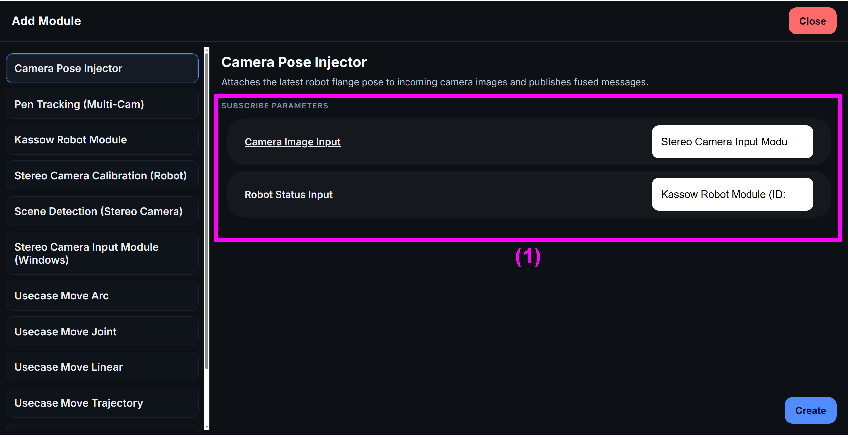
\includegraphics{img/ch5_user_workflow/03_add_injector.pdf}
  \caption[Module input mapping]{Module input mapping example: \emph{Camera Pose Injector} consumes the camera stream and robot status; in the demonstrated setup the mapping is auto-filled.}
  \label{fig:ch5_input_mapping}
\end{figure}

\minihead{Input mapping (when shown).}
Most modules consume outputs of other modules and therefore show an input mapping panel \uicall[fig:ch5_input_mapping]{1}.
In the demonstrated configuration, each input has a single compatible producer at the time the module is added, so the mapping is filled automatically and can be left unchanged.
If the mapping is not filled automatically, the current module set does not match this tutorial; return to \emph{Setup Modules}, remove unexpected instances, and continue by following the module list in the stated order.

% ----------------------------------------------------------
\section{Activation and calibration}
\label{sec:ch5_activation_calibration}

\minihead{Activate the stereo camera module.}
In \emph{Setup Modules}, select \emph{Stereo Camera Input Module (Windows)} (\uicall{1}), keep the default parameters for the thesis hardware, and press \uicall{2} \emph{Activate} (\autoref{fig:ch5_activate_camera_robot}).
If activation fails, verify that the OS can access the camera and re-check the selected resolution and frame rate.

\minihead{Activate the robot module.}
Select \emph{Kassow Robot Module} (\uicall{3}), set \uicall{4} \emph{Host} to the robot controller IP address, and press \uicall{5} \emph{Activate} (\autoref{fig:ch5_activate_camera_robot}).
A wired Ethernet connection is recommended.

% \begin{figure}[H]
%   \centering
%   \includegraphics[width=\linewidth]{img/ch5_user_workflow/fig_ch5_03_activate_camera_robot.pdf}
%   \caption[Activating camera and robot]{Activating the camera and robot modules in \emph{Setup Modules}.}
%   \label{fig:ch5_activate_camera_robot}
% \end{figure}

\minihead{Calibrate the robot-mounted stereo rig.}
Select \emph{Stereo Camera Calibration (Robot)}.
For each list entry (\uicall{1}), press \uicall{2} \emph{Click to set} to capture one synchronized sample (stereo image + flange pose), and use \uicall{3} to add more entries as needed (\autoref{fig:ch5_calib_inputs}).
Capture at least 10 samples while:
(i) the Charuco board is static, flat, and visible in both cameras, and
(ii) the robot pose changes significantly between captures (vary position and orientation).

After collecting samples, press \uicall{4} \emph{Activate} to run calibration.
If calibration fails, the captured dataset likely did not contain enough sharp, well-lit, diverse stereo views of the board (simultaneously visible in both cameras) or did not contain enough robot motion diversity; capture more samples with larger board coverage and stronger pose variation and retry.

% \begin{figure}[H]
%   \centering
%   \includegraphics[width=\linewidth]{img/ch5_user_workflow/fig_ch5_04_calibration_inputs.pdf}
%   \caption[Providing calibration captures]{Providing calibration captures in the activation UI.}
%   \label{fig:ch5_calib_inputs}
% \end{figure}

\minihead{Save the setup (recommended).}
To persist the current module graph and module state, press \emph{Save} in \emph{Setup Modules} and confirm the save name in the dialog.
\xxx{Optionally add 1 small figure for the Save dialog if you keep this section. Otherwise keep as text.}

% ----------------------------------------------------------
\section{Main view essentials (what the operator needs)}
\label{sec:ch5_main_view}

Close \emph{Setup Modules} to return to the \emph{Aergo} main view (\autoref{fig:ch5_main_view}).
The main view shows a camera preview and a shared 3D visualization, plus the use case program panel.

% \begin{figure}[H]
%   \centering
%   \includegraphics[width=\linewidth]{img/ch5_user_workflow/fig_ch5_05_main_view_pen.pdf}
%   \caption[Main view and pen interaction]{Main view and pen interaction.}
%   \label{fig:ch5_main_view}
% \end{figure}

\minihead{3D navigation.}
Drag with the left mouse button to rotate, right mouse button to pan, and use the mouse wheel to zoom.

\minihead{Wake the pen and test pose/trajectory capture.}
Wake the pen by shaking it; it should advertise over BLE as \type{"3D Pen"}.
Keep the marker cube visible in the camera preview; the tracked pen pose appears in the 3D view (\uicall{1}).
\begin{itemize}
  \item \textbf{Pose:} press the \emph{primary} button briefly to create a pose marker (\uicall{2}).
  \item \textbf{Trajectory:} press and hold the primary button, move the pen, then release to create a trajectory preview (\uicall{3}).
\end{itemize}

\minihead{Set Position / Move To Position (safety).}
\emph{Set Position} stores the current robot joint configuration as a convenient home pose; \emph{Move To Position} commands a move to the stored pose.
\xxx{Add a 1--2 sentence safety note: keep workspace clear; be ready to hit E-stop before commanding motion.}

\minihead{Two utility actions (short notices).}
\begin{itemize}
  \item \textbf{Scan Scene:} refreshes the displayed box detections by triggering one scene snapshot.
  \item \textbf{Reload Visualization:} clears and rebuilds the UI-local visualization if stale artifacts remain visible.
\end{itemize}

% ----------------------------------------------------------
\section{User story: pick-and-place}
\label{sec:ch5_story_pick_place}

\minihead{Goal.}
Pick a detected box near an authored pick pose and place it at an authored place pose.

\minihead{Precondition (scene).}
At least one fiducial-tagged box must be visible to the camera (registry in \autoref{appendix:scene_registry}).

\minihead{Steps.}
\begin{enumerate}
  \item In \emph{Available}, press \uicall{1} \emph{PICK}. The use case appears in the \emph{Program} list (\uicall{2}) and its parameters are shown (\uicall{3}).
  \item Trigger auto-loading by pressing the pen \emph{secondary} button.
        The UI first acquires a scene snapshot and then prompts for the pick and place poses.
  \item Enter \emph{Pick Position} by moving the pen tip close to the intended box and pressing the primary button.
  \item Enter \emph{Place Position} by moving the pen to the target location and pressing the primary button.
  \item Press \uicall{4} \emph{Confirm}. If confirmation fails (no object near the pick pose), reteach \emph{Pick Position}.
  \item Press \uicall{5} \emph{Start} to execute. Stop is supported; pause is not supported by this use case.
\end{enumerate}

% \begin{figure}[H]
%   \centering
%   \includegraphics[width=\linewidth]{img/ch5_user_workflow/fig_ch5_06_pick_before_after.pdf}
%   \caption[Pick-and-place programming]{Pick-and-place programming (before/after confirmation).}
%   \label{fig:ch5_pick_before_after}
% \end{figure}

\noindent \minihead{Note.}
Pick-and-place re-reads the scene at execution start; the preview shown after confirmation is illustrative.

% ----------------------------------------------------------
\section{User story: weld}
\label{sec:ch5_story_weld}

\minihead{Goal.}
Create and execute a weld command by (i) scanning the scene and (ii) drawing a trajectory along an intended seam.

\minihead{Precondition (scene).}
Place two tagged boxes so that they touch (edge--edge or edge--face contact).
The weld use case detects seam candidates from the current box configuration and matches the user-drawn trajectory to one seam.

\minihead{Steps.}
\begin{enumerate}
  \item In \emph{Available}, press \uicall{1} \emph{WELD}. The use case appears in the \emph{Program} list (\uicall{2}) and its parameters are shown (\uicall{3}).
  \item For \emph{Scene Scan}, press \uicall{4} \emph{Click to set} to acquire a scene snapshot. Detected boxes appear in the 3D view (\uicall{5}).
  \item For \emph{Welding Trajectory}, press \uicall{6} \emph{Click to set}. When prompted, draw a trajectory along the intended seam (press and hold primary, move, release).
  \item Press \uicall{7} \emph{Confirm}. If command creation fails (trajectory cannot be matched to a seam), remove the trajectory value and reteach; if boxes were moved, refresh \emph{Scene Scan}.
  \item Press \uicall{8} \emph{Start} to execute. Pause and stop are supported by this use case.
\end{enumerate}

% \begin{figure}[H]
%   \centering
%   \includegraphics[width=\linewidth]{img/ch5_user_workflow/fig_ch5_07_weld_before_after.pdf}
%   \caption[Weld programming]{Weld programming (before/after confirmation).}
%   \label{fig:ch5_weld_before_after}
% \end{figure}

\noindent \minihead{Note.}
Unlike pick-and-place, the weld command is resolved at confirmation time and assumes the workpiece configuration remains unchanged until execution.

% ----------------------------------------------------------
\section{Persistence workflows (optional)}
\label{sec:ch5_persistence}

\minihead{Save/load setup.}
Use \emph{Setup Modules → Save/Load} to persist the module graph and per-module state (\autoref{sec:ch3_persistence_semantics}).

\minihead{Save/load program.}
Use \emph{Main view → Save/Load} to persist the authored command list and parameter values (\autoref{sec:ch3_persistence_semantics}).

\xxx{Optional 1 figure: one combined Save/Load dialog screenshot; otherwise keep text-only.}